\documentclass[12pt,a4paper]{book}

% ----- Encodage & langues -----
\usepackage[utf8]{inputenc}    % Encodage UTF-8
\usepackage[T1]{fontenc}       % Meilleure gestion des accents
\usepackage[french]{babel}     % Langue du document (français)

% ----- Police -----
\usepackage{lmodern}           % Police Latin Modern (propre et lisible)
%\usepackage{mathpazo}         % Option : police Palatino
%\usepackage{times}            % Option : police Times

% ----- Mise en page -----
\usepackage[a4paper,margin=2.5cm]{geometry} % Marges

% ----- Liens cliquables -----
\usepackage[hidelinks]{hyperref} % Liens URL et références
\hypersetup{
    colorlinks=true,
    linkcolor=blue,
    urlcolor=cyan,
    citecolor=red
}

% ----- Table des matières -----
\setcounter{tocdepth}{2} % Profondeur de la ToC (sections, sous-sections, etc.)

% ----- Autres utiles -----
\usepackage{graphicx}     % Pour insérer des images
\usepackage{amsmath,amssymb} % Maths
\usepackage{enumitem}     % Listes personnalisées
\usepackage{fancyhdr}     % En-têtes et pieds de page
\usepackage{setspace}     % Interligne
\onehalfspacing           % Interligne 1.5
\usepackage{titling}
\usepackage{epigraph}
\usepackage[most]{tcolorbox}
\usepackage{xcolor}
\usepackage{mdframed}
\usepackage{textcomp}

% Définition d'une citation décorative
\newmdenv[
    backgroundcolor=gray!8,    % Fond gris très clair
    linewidth=0pt,             % Pas de bordure
    leftmargin=0pt,            % Supprime les marges automatiques
    rightmargin=0pt,
    innerleftmargin=2em,       % Marge interne gauche
    innerrightmargin=2em,      % Marge interne droite
    innertopmargin=1em,
    innerbottommargin=1em,
    roundcorner=5pt,
    font=\itshape\centering,   % Italique et centré
    align=center,              % Centre la boîte elle-même
    userdefinedwidth=0.7\textwidth  % Largeur définie (70% du texte)
]{citationmd}


% ----- Début du document -----

\begin{document}

\begin{titlepage}
    \centering
    \vspace*{1cm}
    \Huge
    \textbf{L'Odyssée de l'Intelligence Artificielle}
    
    \begin{figure}[h]
        \centering
        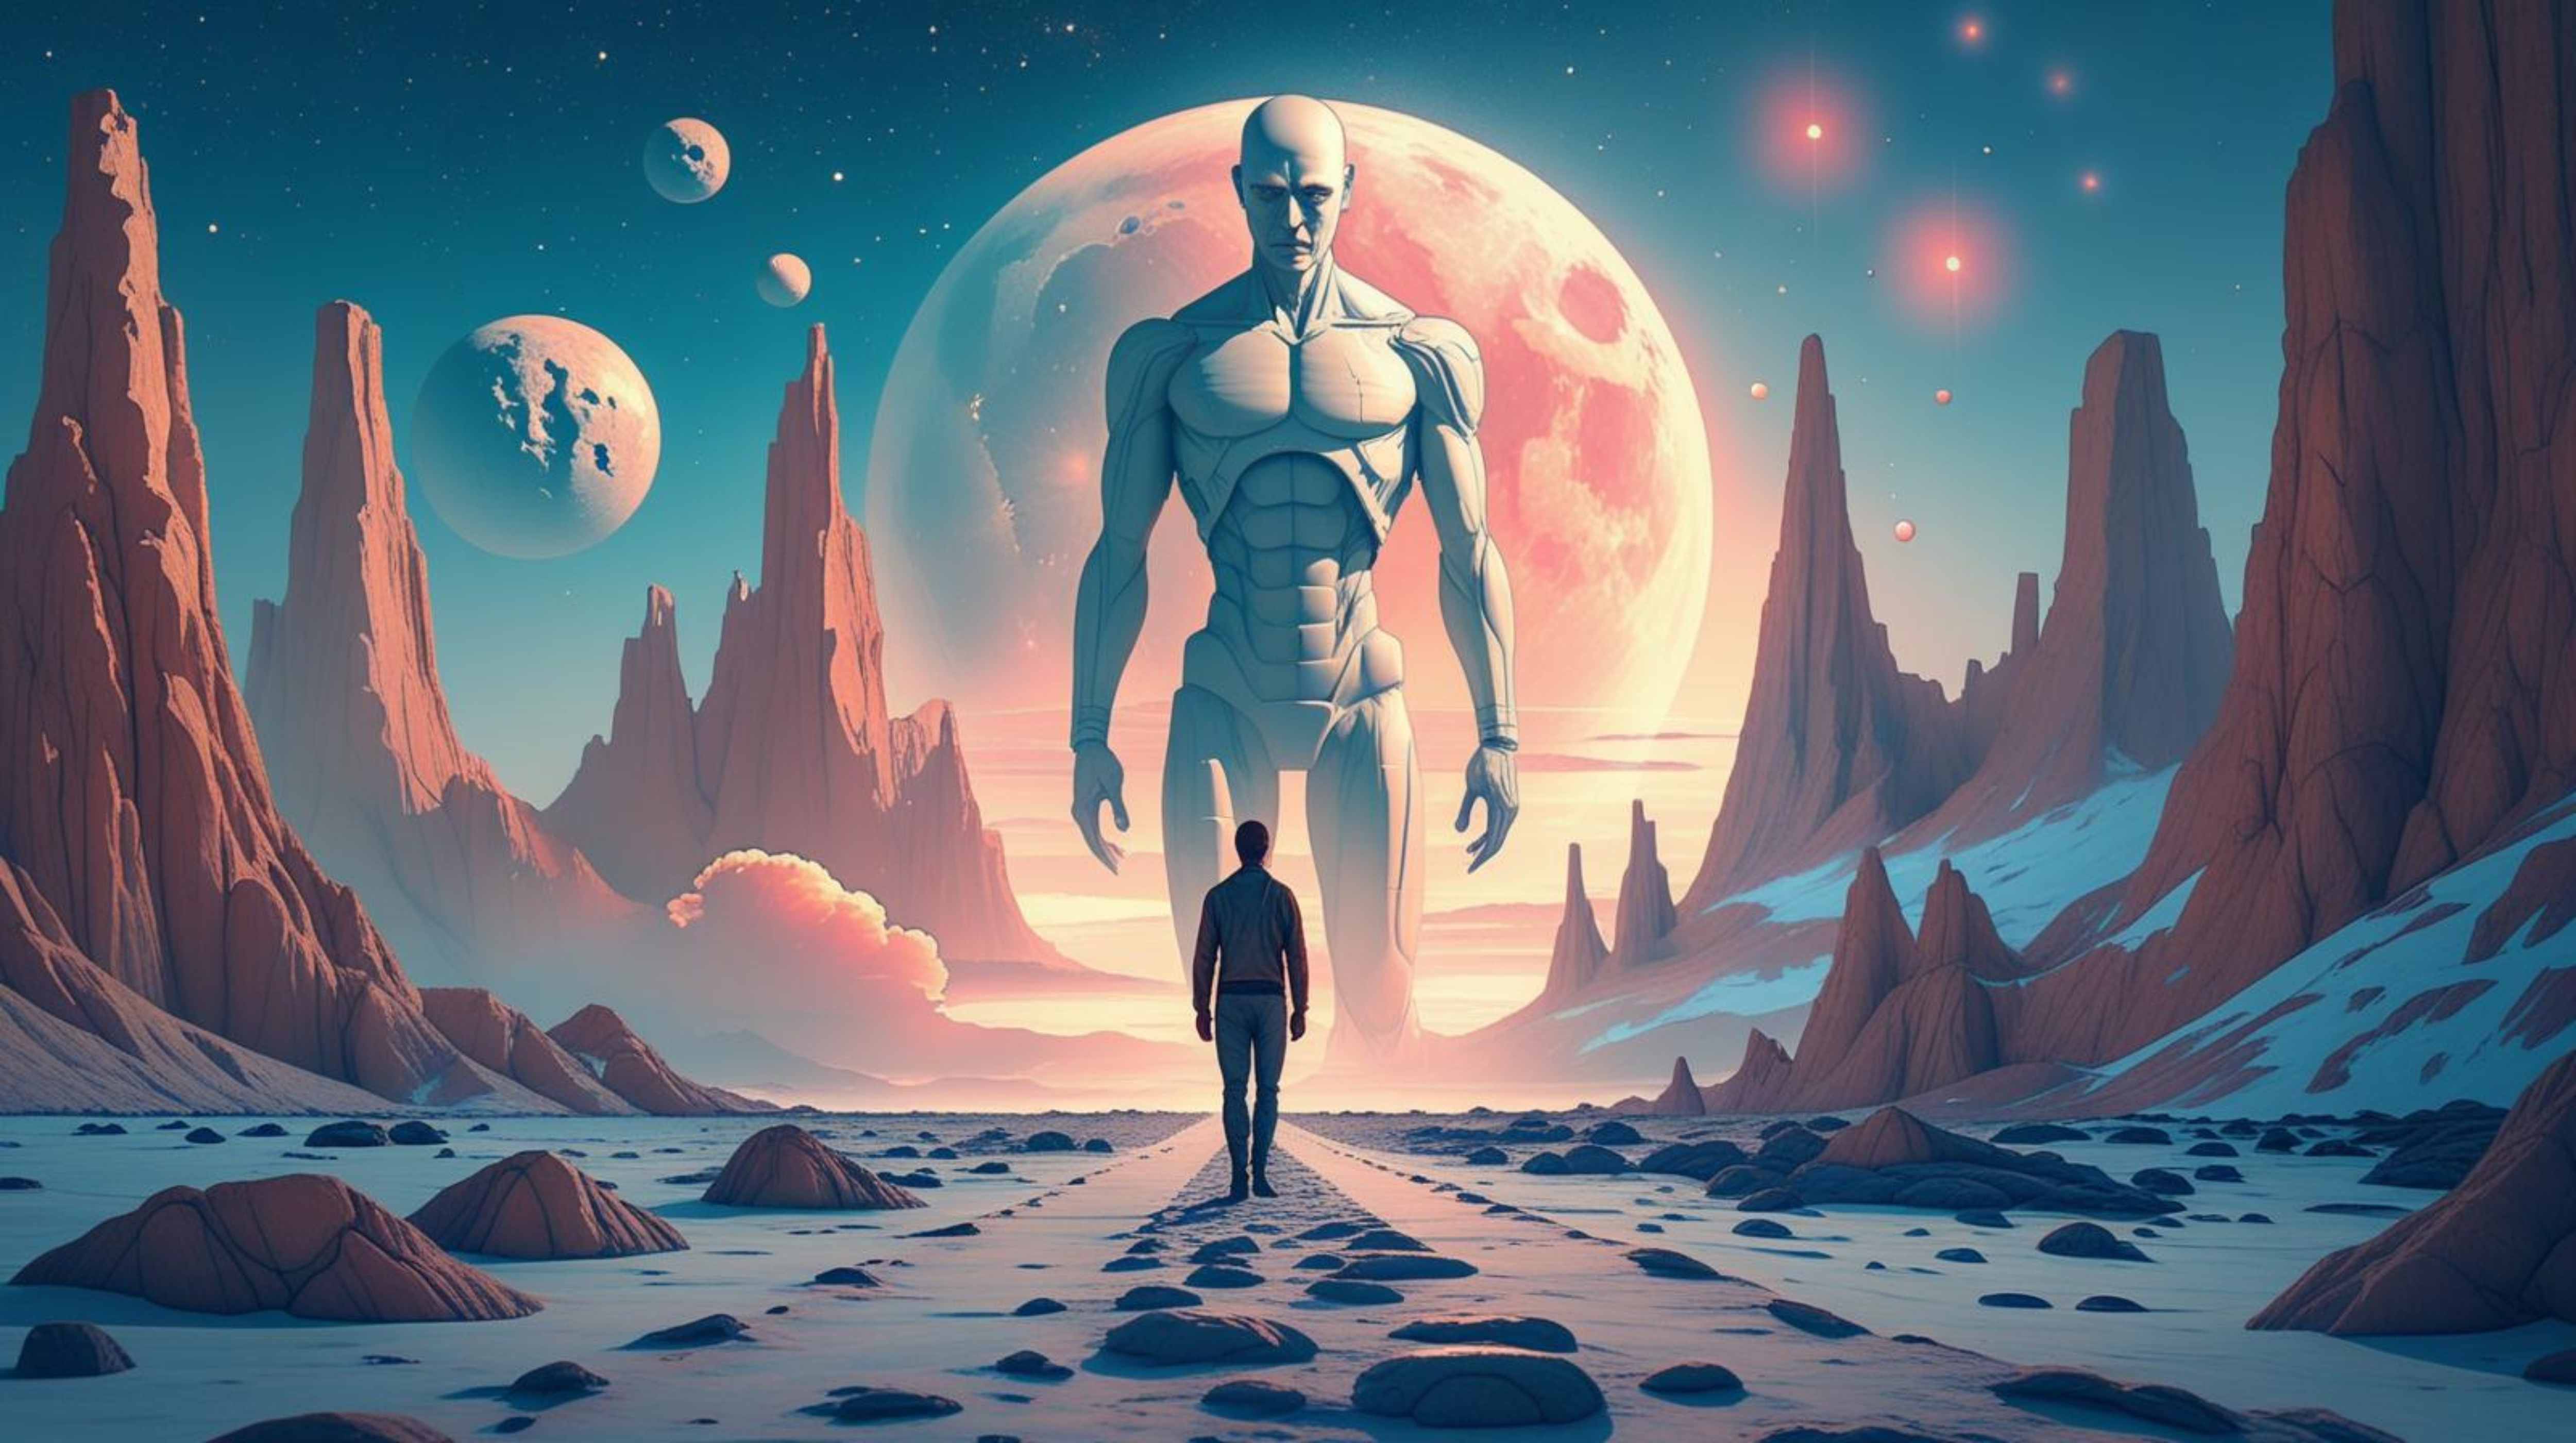
\includegraphics[width=1\textwidth]{images/partie1/odysse.png}
    \end{figure}

    \vspace{0.5cm}
    
    \LARGE
    \textit{Des Origines Anthropologiques aux Horizons Contemporains}
    
    \vspace{2cm}

    \Large
    Romuald Courtois
    
    \vspace{2cm}
            
    \large
    2025

\end{titlepage}

\newpage
\pagestyle{empty}

\begin{center}
2025 Romuald Courtois

\bigskip

Tous droits réservés. Aucune partie de ce livre ne peut être reproduite, stockée dans un système de récupération, ou transmise sous aucune forme ni aucun moyen, électronique, mécanique, photocopie, enregistrement ou autre, sans l'autorisation écrite préalable de l'auteur, sauf dans les cas prévus par la loi (citations, critiques, usages pédagogiques).

\bigskip

ISBN : [Votre numéro ISBN]

\bigskip

Dépôt légal : 23/09/2025

\bigskip

Édition : Auto-édition

\bigskip

Adresse de l'auteur / de l'éditeur :\\
151 Traverse de la Gouffonne, 13009 MARSEILLE

\bigskip

Pour obtenir une autorisation de reproduction ou pour toute question relative aux droits, veuillez contacter :\\
romuald.courtois.at.proton.me

\bigskip

Les noms de marques, logos, produits ou institutions mentionnés dans ce livre sont la propriété de leurs détenteurs respectifs.

\bigskip

La couverture a été réalisée par : Romuald Courtois
\end{center}

\newpage
\pagestyle{empty}
\chapter*{Préface} % Titre sans numéro
\addcontentsline{toc}{chapter}{Préface}  % Ajoute la préface à la table des matières
Dans chaque avancée technologique, dans chaque progrès de la pensée humaine, se cache un paradoxe fascinant : celui de l'éternel fainéant ambitieux. Ce livre s'articule autour de cette idée directrice, selon laquelle l'humanité, portée par une ambition immense, cherche depuis toujours à alléger ses efforts par l'externalisation de ses capacités — qu'elles soient physiques, intellectuelles ou créatives. Nous sommes à la fois poussés par la paresse, ce désir de faciliter notre quotidien, et par une soif infinie d'innovation, de conquête intellectuelle.
\\ \\
L'histoire de l'intelligence artificielle est de fait une illustration parfaite de ce double mouvement. Depuis les premiers automates antiques jusqu'aux réseaux neuronaux profonds d'aujourd'hui, cette quête révèle non seulement notre envie d'économiser l'énergie humaine, mais aussi notre rêve de transcender nos limites cognitifs. Ce livre retrace cette odyssée passionnante, mêlant récits historiques, analyses techniques et réflexions éthiques.
\\ \\
À travers la figure de ce "fainéant ambitieux", j'espère porter un regard à la fois critique et bienveillant sur les innovations majeures, en montrant comment chaque invention est à la fois un outil pour réduire l'effort et un levier d'ambition démesurée. Il invite le lecteur à comprendre que derrière chaque progrès, derrière chaque machine intelligente, il y a une humanité impatiente qui cherche inlassablement à se simplifier la vie… tout en repoussant ses propres frontières.
\\ \\
Que cet ouvrage nourrisse la curiosité, stimule la réflexion et éclaire le chemin vers une intelligence artificielle enfin alignée avec nos valeurs et nos besoins profonds.
\\ \\
\begin{citationmd}
\centering\itshape\large
"L'homme est un éternel fainéant ambitieux : trop paresseux pour accepter la répétition, trop intelligent pour accepter l'inefficacité. C'est cette contradiction qui nous a menés de l'outil de pierre aux neurones artificiels."
\end{citationmd}
 
\pagestyle{empty}
\tableofcontents

\newpage
\pagestyle{plain}
\chapter*{Introduction}
\addcontentsline{toc}{chapter}{Introduction}

L'intelligence artificielle, souvent perçue comme une révolution contemporaine, est en réalité l'aboutissement d'une quête profondément ancrée dans l'histoire même de l'humanité, bien avant l'invention des premiers outils sophistiqués. Pour comprendre pleinement cette trajectoire, il faut remonter jusqu'aux origines de notre espèce, à ce moment clé où nos ancêtres ont commencé à se redresser, posant ainsi les premières pierres d'un cheminement qui allait transformer non seulement leur corps, mais aussi leur esprit.
\\ \\
Le passage à la bipédie, il y a plus de 4 millions d'années, a libéré les mains tout en stimulant les possibilités cognitives, ouvrant la voie à la fabrication d'outils rudimentaires. Ces premières externalisations des fonctions physiques incarnent déjà la dynamique que l'on retrouve dans l'intelligence artificielle : réduire la charge corporelle ou mentale par l'usage d'artefacts externes. Cette ambition de « paresse créative » est à l'origine de toutes les technologies, et en filigrane de l'émergence des processus cognitifs complexes qui caractérisent notre espèce.
\\ \\
Ce livre propose donc de retracer l'odyssée de l'IA en partant de ce moment fondamental où l'humanité s'est levée, au propre et au figuré, jusqu'aux dernières innovations numériques actuelles. Il s'agit d'un voyage mêlant anthropologie, technologie, philosophie et éthique, qui éclaire comment, à chaque époque, le désir d'alléger l'effort s'est conjugué à une ambitieuse vision d'extension des capacités humaines. 
\\ \\
À travers la notion de \textit{"l'éternel fainéant ambitieux"}, vous découvrirez comment cette dualité originelle continue de guider nos inventions et leurs implications. Ce n'est pas seulement une histoire de machines, mais celle du regard humain sur lui-même, sur ses potentialités et ses limites. 
\\ \\
Bienvenue dans cette plongée aux origines, à la source de toute intelligence, humaine et artificielle.

\newpage
\part{GENÈSE ET FONDEMENTS HISTORIQUES}

\chapter{Genèse Anthropologique - L'Éveil du Fainéant}
\section{Bipédie et libération cognitive (4 Ma - 200 000 ans)}
\section{Premiers outils lithiques et externalisation motrice}
\section{Révolution cognitive et pensée symbolique (70 000 - 10 000 ans)}
\section{Néolithique, spécialisation et division du travail}

\chapter{Civilisations Antiques et Mécanisation Primitive}
\section{Mésopotamie - Calculs, abaques et premiers algorithmes}
\section{Égypte - Mathématiques, ingénierie et automatisation}
\section{Grèce - Logique, philosophie et automates mécaniques}
\section{Rome - Ingénierie, hydraulique et machines complexes}

\chapter{Synthèses Orientales et Renaissance Islamique}
\section{Inde - Mathématiques, logique et premiers concepts algorithmiques}
\section{Chine ancienne - Boulier, poudre et automates mécaniques}
\section{Islam - Traductions, mathématiques et premiers ordinateurs mécaniques}
\section{Transmission vers l'Europe - Textes, écoles et premiers penseurs}

\chapter{Renaissance Européenne et Révolution Scientifique}
\section{Léonard de Vinci - Automates et machines programmables}
\section{Révolution astronomique - Kepler, calculs et précision}
\section{Pascal et Leibniz - Premières machines à calculer}
\section{Newton et la mathématisation du monde}

\chapter{Siècle des Lumières et Mécanisation}
\section{Automates de Vaucanson et illusion de vie}
\section{Encyclopédie et diffusion des techniques}
\section{Révolution industrielle - Métiers mécaniques et automation}
\section{Jacquard - Programmation par cartes perforées}


\chapter{XIXe Siècle - Émergence de l'Information}
\section{Babbage et Lovelace - Machines analytiques}
\section{Boole - Algèbre logique et fondements booléens}
\section{Maxwell, thermodynamique et théorie de l'information}
\section{Télégraphie, codes et transmission}

\part{NAISSANCE ET DÉVELOPPEMENT DE L'IA MODERNE}
\chapter{XXe Siècle - Fondements Théoriques}
\section{Hilbert et formalisme mathématique}
\section{Gödel - Limites de la démonstration automatique}
\section{Turing - Calculabilité et machines universelles}
\section{Von Neumann - Architecture et automates cellulaires}

\chapter{Naissance Officielle de l'IA (1940-1960)}
\section{McCulloch-Pitts et neurones formels}
\section{Wiener et cybernétique}
\section{Shannon et théorie de l'information}
\section{Conférence de Dartmouth et manifeste fondateur}

\chapter{Première Génération - Optimisme Symbolique}
\section{Logic Theorist et résolution automatique}
\section{Perceptron et apprentissage connexionniste}
\section{LISP et programmation symbolique}
\section{Premiers systèmes experts et bases de connaissances}

\chapter{Premier Hiver et Remises en Question (1970-1980)}
\section{Rapport Lighthill et crise de confiance}
\section{Limites des perceptrons (Minsky-Papert)}
\section{Complexité computationnelle et problèmes NP}
\section{Échec des promesses et réduction des financements}

\chapter{Renaissance des Systèmes Experts (1980-1990)}
\section{MYCIN et diagnostic médical automatisé}
\section{DENDRAL et analyse chimique}
\section{Ingénierie de la connaissance et ontologies}
\section{Marché commercial et désillusions}

\chapter{Révolution Statistique et Second Hiver}
\section{Réseaux de neurones et rétropropagation}
\section{Réseaux bayésiens et raisonnement probabiliste}
\section{Machine Learning et approches data-driven}
\section{Deep Blue vs Kasparov - Calcul brut vs intuition (1997)}

\part{RÉVOLUTION CONTEMPORAINE ET IMPACTS SOCIÉTAUX}
\chapter{Internet et Renaissance des Données (2000-2010)}
\section{Web sémantique et ontologies distribuées}
\section{Big Data et nouveaux paradigmes d'apprentissage}
\section{Google et PageRank - IA comme service}
\section{Réseaux sociaux et intelligence collective}

\chapter{Deep Learning et Révolution Connexionniste}
\section{AlexNet et renaissance des CNN (2012)}
\section{GANs et génération de contenu artificiel}
\section{RNN, LSTM et modélisation séquentielle}
\section{Révolution Transformers et mécanismes d'attention}

\chapter{IA Générative et Démocratisation (2017-2025)}
\section{GPT et génération de texte à grande échelle}
\section{DALL-E et création d'images automatisée}
\section{ChatGPT et interface conversationnelle grand public (2022)}
\section{Codex et programmation assistée par IA}

\chapter{Succès Médiatisés et Révolutions Sectorielles}
\section{Netflix Recommandations - Révolution de la personnalisation (2006)}
\section{AlphaGo vs Lee Sedol - Maîtrise du jeu de Go (2016)}
\section{AlphaFold - Révolution en biologie structurale (2020)}
\section{GitHub Copilot - IA collaborative en programmation (2021)}

\chapter{Échecs Médiatisés et Leçons Critiques}
\section{Accident Tesla Autopilot - Limites de la conduite autonome (2016)}
\section{Tay de Microsoft - Dérapage raciste en 24h (2016)}
\section{Reconnaissance faciale biaisée - Amazon Rekognition (2018)}
\section{Zillow iBuying - Algorithmes immobiliers défaillants (2021)}
\section{ChatGPT et hallucinations juridiques (2023)}
\section{McDonald's Drive-AI - Abandon commercial (2024)}

\chapter{IA Militaire et Géopolitique}
\section{Systèmes d'armes autonomes (LAWS) et débat éthique}
\section{Cyberguerre et IA défensive/offensive}
\section{Course géopolitique USA-Chine-Europe}
\section{Surveillance de masse et contrôle social}

\part{DIMENSIONS HUMAINES ET PROSPECTIVE}
\chapter{Approches Bio-Inspirées et Active Inference}
\section{Friston et Free Energy Principle}
\section{Active Inference et anticipation prédictive}
\section{Neurosciences computationnelles et modélisation cérébrale}
\section{Réseaux de neurones évolutionnistes}

\chapter{Facteurs Humains et Ergonomie Cognitive}
\section{IHM et interfaces adaptatifs}
\section{Lecture des intentions par eye-tracking}
\section{Cognition énactive et robotique incarnée}
\section{Charge cognitive et optimisation des performances}

\chapter{Interfaces Cerveau-IA et Augmentation Cognitive}
\section{Neuralink et interfaces implantées - Progrès et risques}
\section{Délestage cognitif - Dépendance et atrophie des capacités}
\section{IA thérapeutique - Santé mentale, autisme, réhabilitation}
\section{Biais cognitifs humains reproduits par l'IA}

\chapter{Les Oubliés de la Révolution IA}
\section{Pionniers invisibles - Femmes en IA (Ada Lovelace revisitée)}
\section{Contributeurs non-occidentaux souvent occultés}
\section{Populations rurales et seniors face à l'IA}
\section{Travailleurs du clic et main-d'œuvre cachée}

\chapter{Transformation Sociétale et Économique}
\section{Remplacement d'emplois et nouvelles professions}
\section{Fracture numérique et inégalités d'accès}
\section{IA générative et propriété intellectuelle}
\section{Économie de l'attention et manipulation comportementale}

\chapter{IA Créative et Patrimoine Culturel}
\section{IA générative artistique - DALL-E, Midjourney, Stable Diffusion}
\section{Littérature et IA - GPT-poetry, co-écriture}
\section{Préservation du patrimoine - Numérisation, restauration virtuelle}
\section{Déformation historique - Risques pour la mémoire collective}

\chapter{Convergences Technologiques Émergentes}
\section{Informatique quantique et IA - D-Wave, IBM Q}
\section{Technologie quantique : principes et avancées récentes}
\section{IA + Biotechnologies - Drug discovery, thérapies géniques}
\section{IA + Nanotechnologies - Smart materials, médecine régénérative}
\section{Internet des Objets intelligent - Edge computing, IA embarquée}

\chapter{IA et Environnement}
\section{Empreinte carbone de l'IA - Datacenters, consommation énergétique}
\section{IA pour le climat - Modélisation, smart grids, optimisation}
\section{Économie circulaire et IA prédictive}
\section{Obsolescence et e-waste des systèmes IA}

\chapter{Paradigmes Alternatifs et Techniques Redécouvertes}
\section{Techniques pré-deep learning redécouvertes}
\section{IA symbolique hybride - Retour du raisonnement logique}
\section{Bio-computing - ADN, protéines comme processeurs}
\section{IA frugale - Algorithmes low-tech, edge computing}

\chapter{Dérives, Abus et Risques Systémiques de l'IA}
\section{Deepfakes et manipulation de l'information}
\section{Propagation automatisée de la désinformation}
\section{Surveillance de masse et atteintes à la vie privée}
\section{Automatisation des cyberattaques et armes numériques}
\section{Discrimination algorithmique et exacerbation des inégalités}
\section{Effets sur la santé mentale et dépendance aux systèmes IA}

\chapter{Évolution de l'Éthique, Gouvernance et Prospective Finale}
\section{Principes fondateurs et chartes d'intention}
\section{RGPD, AI Act et régulation européenne}
\section{Gouvernance mondiale et coopération internationale}
\section{Justice algorithmique et lutte contre les biais}
\section{Vers l'AGI bio-inspirée et intelligence augmentée}
\section{Black Mirror et dystopies technologiques}
\section{Intelligence collaborative et coévolution}
\section{Vision personnelle - L'odyssée inachevée}
\section{Recommandations pour l'avenir}
\section{Épilogue - Le fainéant ambitieux de demain}



\end{document}